\begin{figure}
\begin{center}
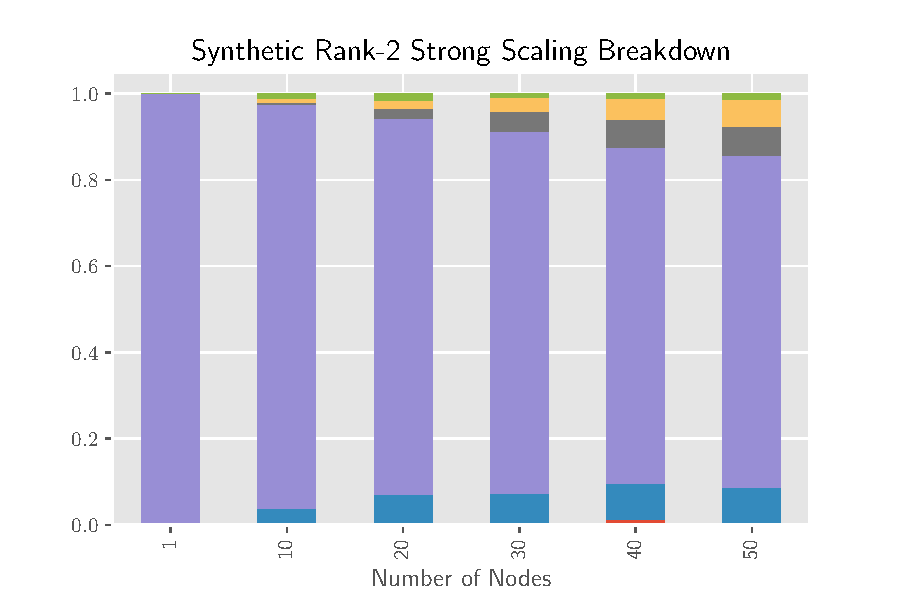
\includegraphics[height=2in, width=\columnwidth]{plots/synthetic_rank2_strongscaling.pdf}
\caption{Relative Time Breakdown for Rank-2 NMF \cref{alg:parrank2nmf} Strong Scaling at Level-0}
\label{fig:synrank2strongscaling}
\end{center}
\end{figure}

\begin{figure}
\begin{center}
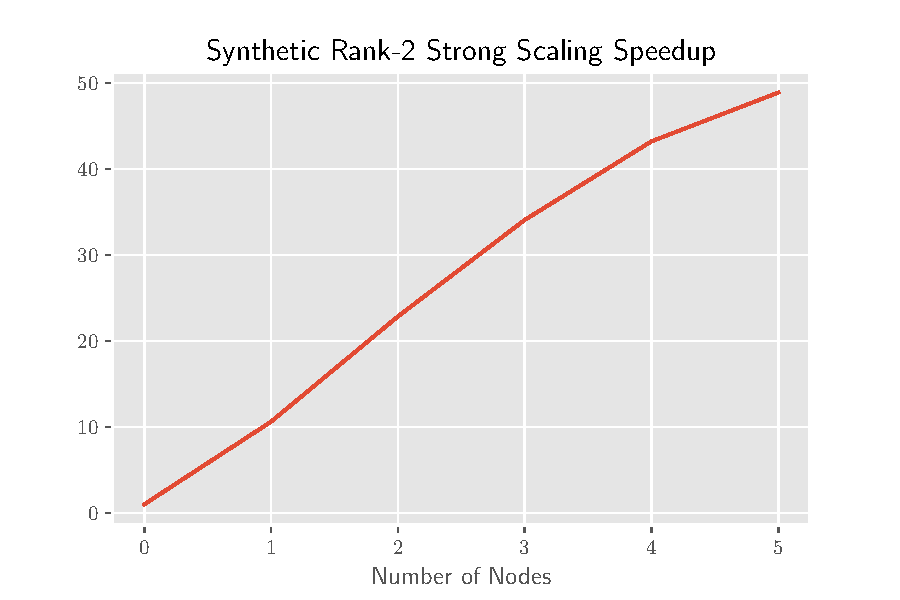
\includegraphics[height=2in, width=\columnwidth]{plots/synthetic_rank2_speedup.pdf}
\caption{Strong Scaling Speedup for Rank-2 NMF \cref{alg:parrank2nmf} at Level-0}
\label{fig:synrank2speedup}
\end{center}
\end{figure}

\begin{figure}
\begin{center}
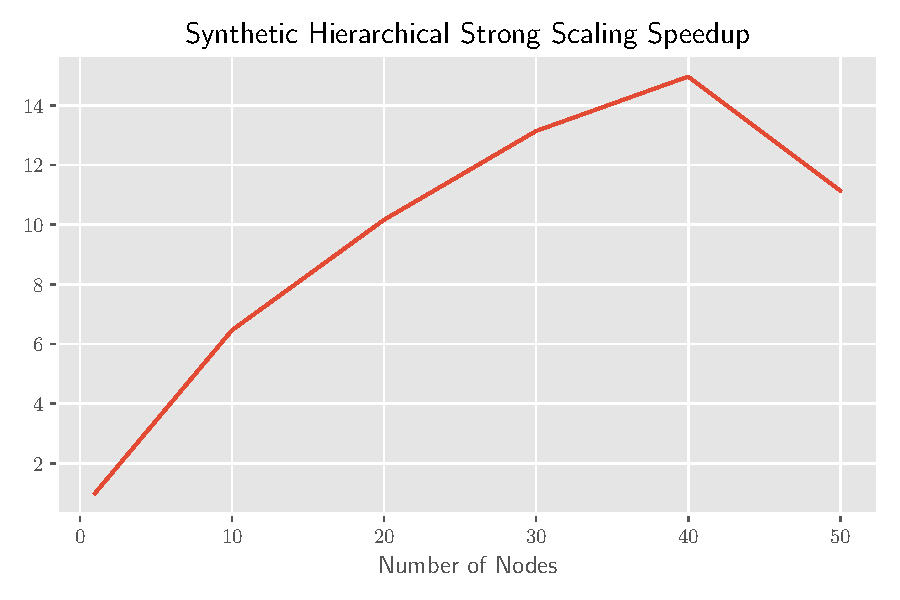
\includegraphics[height=2in, width=\columnwidth]{plots/synthetic_hierarchical_speedup.pdf}
\caption{Strong Scaling Speedup for Hierarchical Clustering. The total time taken for complete Hierarchical Clustering \cref{alg:hiernmf2}}
\label{fig:synhierspeedup}
\end{center}
\end{figure}

\begin{figure}
\begin{center}
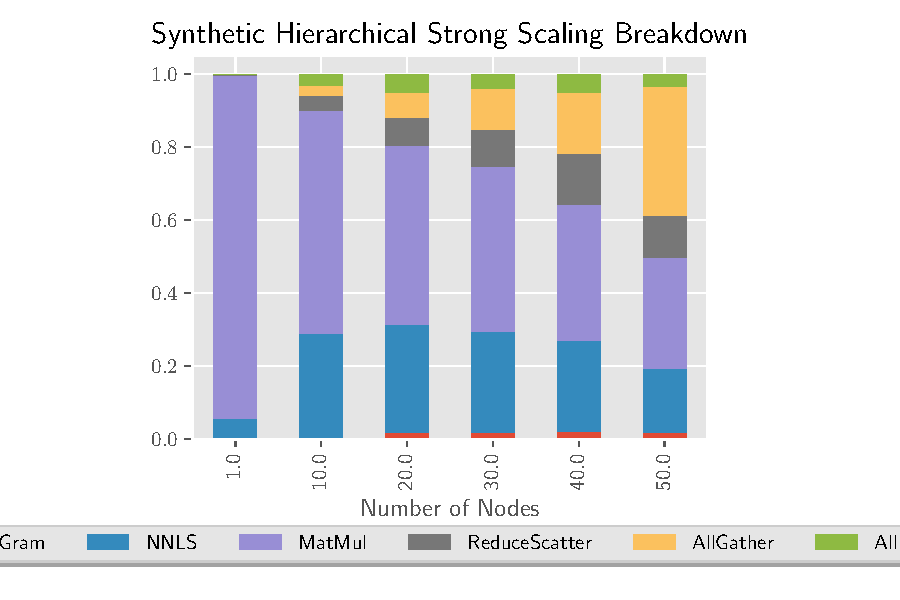
\includegraphics[height=2in, width=\columnwidth]{plots/synthetic_hier_strongscaling.pdf}
\caption{Relative Time Breakdown for Hierarchical Clustering. The plot uses the total time taken for complete Hierarchical Clustering \cref{alg:hiernmf2}}
\label{fig:synhierstrongscaling}
\end{center}
\end{figure}


\begin{figure}
\begin{center}
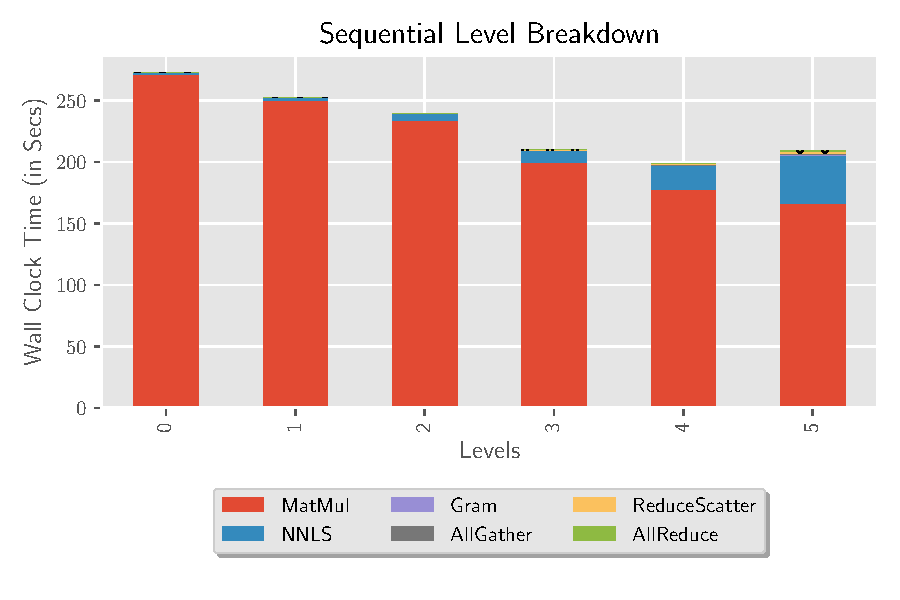
\includegraphics[height=2in, width=\columnwidth]{plots/synthetic_sequential_level_breakdown.pdf}
\caption{Sequential Breakdown plot for levels 0 to 5. y-axis is absolute wall clock time in seconds}
\label{fig:seqlevelbreakdown}
\end{center}
\end{figure}

\begin{figure}
\begin{center}
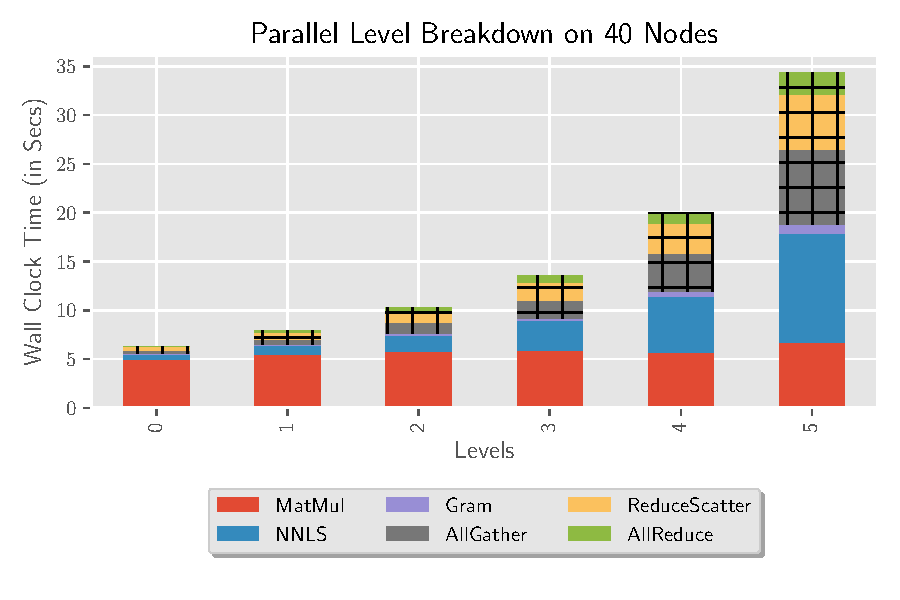
\includegraphics[height=2in, width=\columnwidth]{plots/synthetic_parallel_level_breakdown.pdf}
\caption{Parallel Breakdown plot for levels 0 to 5 on 40 nodes. y-axis is absolute wall clock time in seconds}
\label{fig:parallellevelbreakdown}
\end{center}
\end{figure}